\documentclass{article}
\usepackage[utf8]{inputenc} %кодировка
\usepackage[T2A]{fontenc}
\usepackage[english,russian]{babel} %русификатор 
\usepackage{mathtools} %библиотека матеши
\usepackage[left=1cm,right=1cm,top=2cm,bottom=2cm,bindingoffset=0cm]{geometry} %изменение отступов на листе
\usepackage{amsmath}
\usepackage{graphicx} %библиотека для графики и картинок
\graphicspath{}
\DeclareGraphicsExtensions{.pdf,.png,.jpg}
\usepackage{subcaption}
\usepackage{pgfplots}
\usepackage{float}
\usepackage{graphicx}
\usepackage{hyperref}

\begin{document}

\tableofcontents
\newpage

\section[Перепись]{Перепись}
\subsection[Санта-клаус]{С помощью ИС «Санта-клаус» детям дарят подарки за хорошее поведение. Разработать модель требований, Use-Case модель и доменную модель.}
\subsubsection{Модель требований FURPS+}
Функциональные требования
\begin{itemize}
    \item SEC0 - Система должна обеспечивать регистрацию пользователей с помощью имени пользователя и пароля.
    \item SEC1 - Система должна поддерживать аутентификацию пользователей с помощью имени пользователя и пароля, также может использоваться подтверждения с помощью СМС или email письма.
    \item FR0 - Система должна поддерживать добавления, удаления, редактирование информации (не качества детей) о детях.
    \item FR1 - Система должна обеспечивать возможноть отмечать, удалять поведенческие достижения их детей.
    \item FR2 - Система должна поддреживать просмотр каталога подарков.
    \item FR3 - Система должна поддреживать возможность составления списка интересных подарков для ребёнка.
    \item FR4 - Система должна предоставлять возможность восстановления забытого пароля.
    \item FR5 - Система должна поддреживать редактирование каталога подарков для админов.
\end{itemize}
Нефункциональные требования
\begin{itemize}
    \item USA0 - Система должна обеспечивать адаптивный дизайн для различных устройств.
    \item RELI0 - Система должна быть доступна 99.9\% времени, с автоматическим восстановлением после сбоев.
    \item PERF0 - Система должна обрабатывать тысячи запросов одновременно без существенных задержек.
    \item SUPP0 - Система должна легко масштабироваться для поддержки увеличения числа пользователей.
\end{itemize}
\subsubsection{Use-case диаграмма}
\begin{center}
    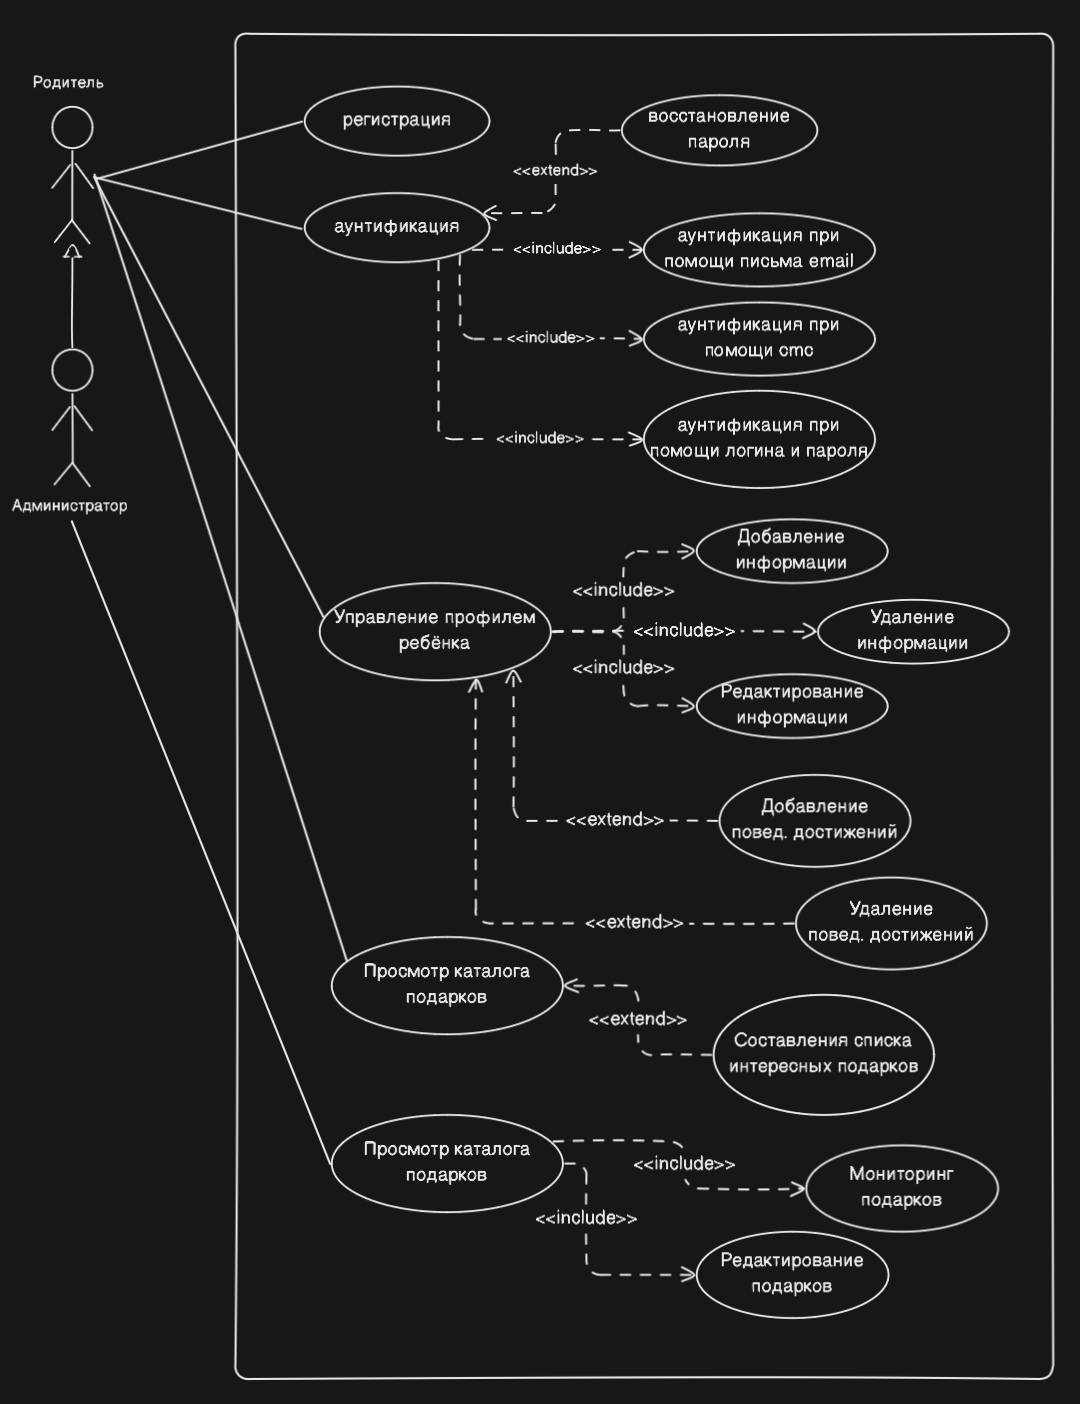
\includegraphics[width=.7\textwidth]{use-case.png}
\end{center}
\subsubsection{Доменная модель}
\begin{center}
    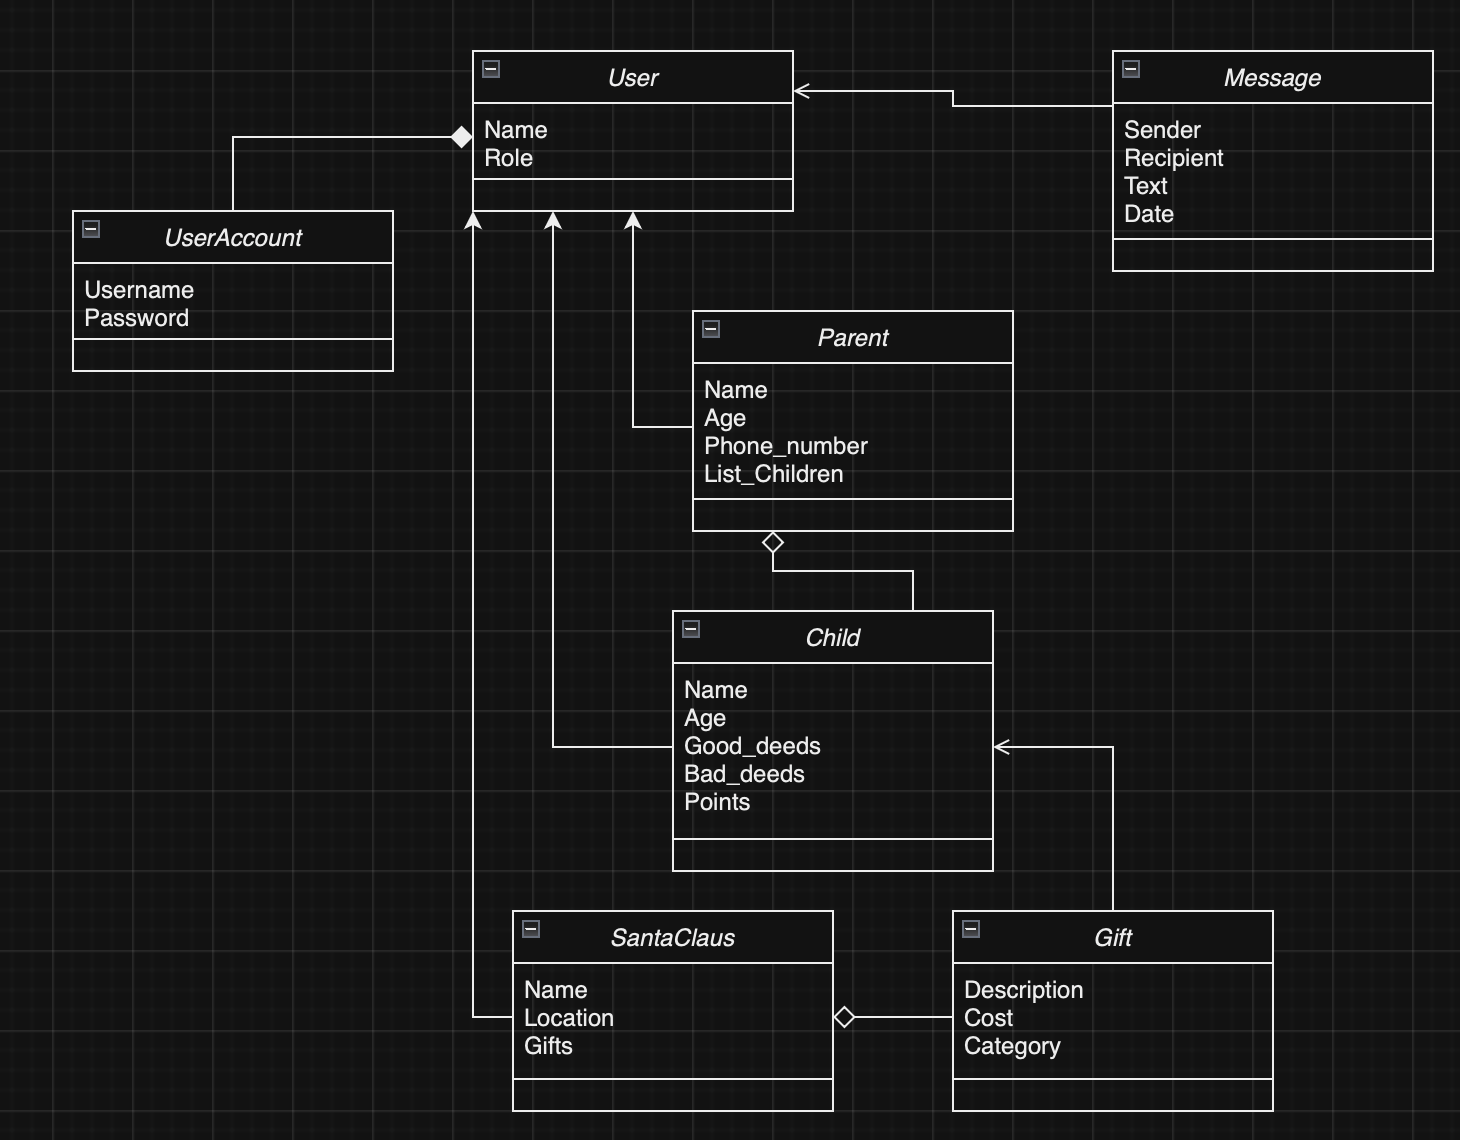
\includegraphics[width=.7\textwidth]{domain_d.png}
\end{center}

\subsection[Disciplined Agile Delivery, +, -]{Модель разработки Disciplined Agile Delivery. «+» и «-» в сравнении с другими моделями}
\subsubsection{Disciplined Agile Delivery}
Модель разработки разработанный Скоттом Амблером, который был вдохновлён системой деления на фазы (начало, построение и внедрение) и подходы как в RUP, но при этом основной цикл разработки посроен на базе гибких методов, включая Scrum. Данная методология является относительно новой на рынке и только развивается.
Так же DAD рассматривает процессы, которые выходят за его собственный процесс разработки
(управление архитектурой и повторным использованием кода, управление персоналом, служба поддержки и текущих операций компании-разработчика, управление портфолио компетенций, непрерывное улучшение процессов разработки и вспомогательных процессов, и многое другое).
\subsubsection{+}
Одним из огромных плюсов (скорее даже это причина появления DAD) - на рынке требовалась методолгия, которая будет комфортна людям, которые, можно сказать, строют марсоход. Они не нуждаются в очень гибких методологиях, так как эти методологии не могут легко маштабироваться на большие команды разработчиков.
Ещё плюсом является то, что можно комбинировать Agile и не Agile подходы в зависимости от требований проекта.
\subsubsection{-}
Минусы: сложность из-за большого количества инструментов и практик, отсюда ватикает следующий минус: высокий уровень компетенций команды для верного построения процессов.

\subsection[Эльфы и тестовое покрытие]{Разработать тестовые сценарии (положительный и отрицательный) для следующего сценария}

-Эльфы получают количество добрых дел у ребенка (К) по его имени и вводят его в систему;

-Если К>=10, то система назначает ему подарок

-Если К<10, то система назначает ему уголек

-Эльф передает назначение на утверждение Санта-Клаусу

Оформить в виде таблицы тестовых случаев (Начальное состояние, ввод пользователя, вывод системы, конечное состояние)
\\ \\
Тест 1:

Начальное состояние: Готово и ожидает получение данных

Ввод пользователя: Иван, 10

Вывод системы: подарок

Конечное состояние: запрос на утверждение у Санта-Клауса
\\ \\
Тест 2:

Начальное состояние: Готово и ожидает получение данных

Ввод пользователя: Иван, 9

Вывод системы: уголёк

Конечное состояние: запрос на утверждение у Санта-Клауса
\\ \\
Тест 3:

Начальное состояние: Готово и ожидает получение данных

Ввод пользователя: Иван, -1

Вывод системы: неверный ввод данных

Конечное состояние: Готово и ожидает получение данных (Начальное состояние)
\\ \\
Тест 4:

Начальное состояние: Готово и ожидает получение данных

Ввод пользователя: Иван, "двадцать один"

Вывод системы: неверный ввод данных

Конечное состояние: Готово и ожидает получение данных (Начальное состояние)

\section[Рубеж]{Вариант - 1}
\subsection{Use-Case}
РАМКА БЕЗ АКТОРОВ!\\
Включение (Include) — обязательная, неотъемлемая связь между use-кейсами.\\
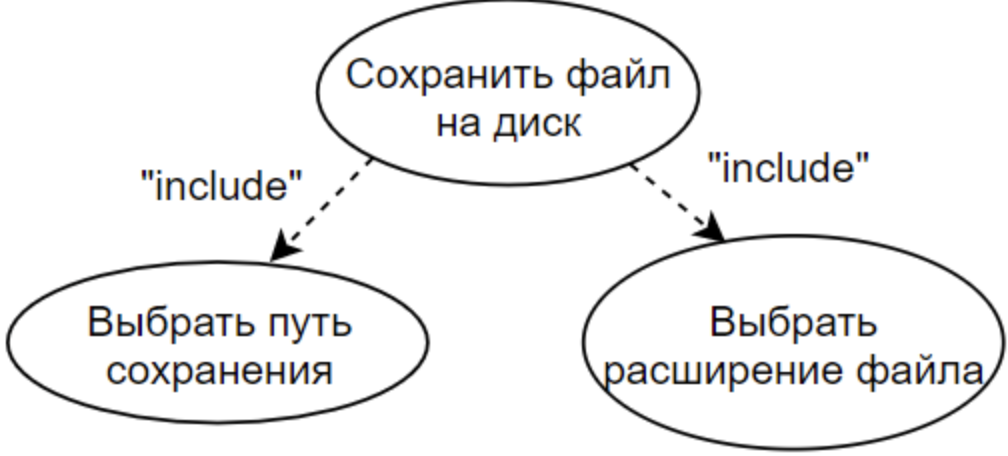
\includegraphics[width=.3\textwidth]{include.png}\\
Расширение (Extend) — необязательное отношение. Если use-кейс не является обязательным, то актор может выбирать.
\\ 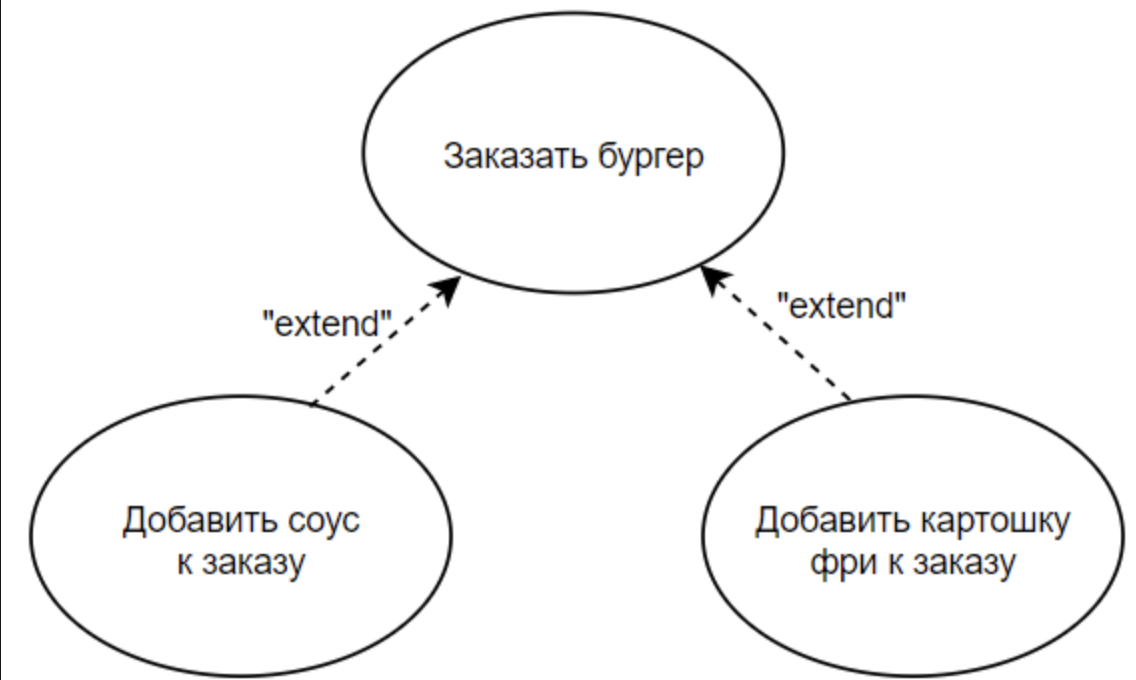
\includegraphics[width=.3\textwidth]{extend.png}\\
Отношение обобщения\\
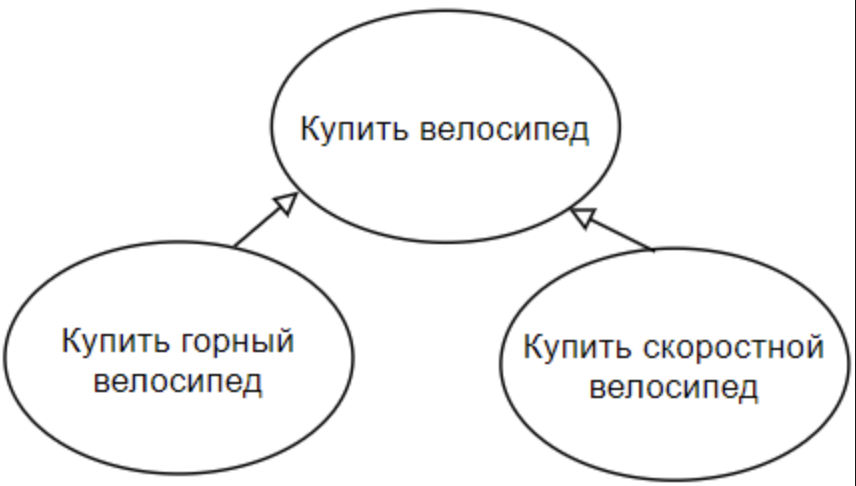
\includegraphics[width=.3\textwidth]{obob.png}\\
Отношение ассоциации\\

\includegraphics[width=.3\textwidth]{assos.png}

\subsection{Модель Ройса}
Если кратко, то он предложил разбиение на следующие шаги:
\begin{itemize}
    \item Предварительный дизайн
    \item Документирование дизайна
    \item Just do it nike tw
    \item Тестирование
    \item Подключение пользователя
\end{itemize}
Подробнее
\begin{itemize}
    \item Предварительный дизайн - занимаются только дизайнеры, цель: спроектировать, определить и создать модели обработки данных, даже если они будут требовать переделок. Разработать док - обзор будущей системы
    \item Документирование дизайна, которое включает: требования к системе, спецификация предварительного
    дизайна, спецификация дизайна интерфейсов, финальные спецификации дизайна системы, план
    тестирования, инструкция по использованию.
    \item Just do it nike tw - Предлагается запустить тестовую разработку параллельно основному процессу и взять это за каскадёра с сокращённым временем разработки, который позволит подтвердить основные хар-ки ПО или найти ошибки. 
    \item Тестирование - наиболее рискованная и дорогостоящая фаза, а также последний шанс для выбора альтернатив. Также при планировании тестирования исключается дизайнер и осмотр всех логических путей проводит другое лицо для инспекции кода. После исправления ошибок нужно провести checkout (тестирование)
    \item Подключение пользователя - это должно произойти на ранних этапах перед финальной поставкой продукта. Необходимо 3 точки: опыт, оценка и подтверждение пользователем - предварительный, критический и финальный просмотр.
\end{itemize}

\subsection{Тестовое покрытие с использованием анализа эквивалетности}
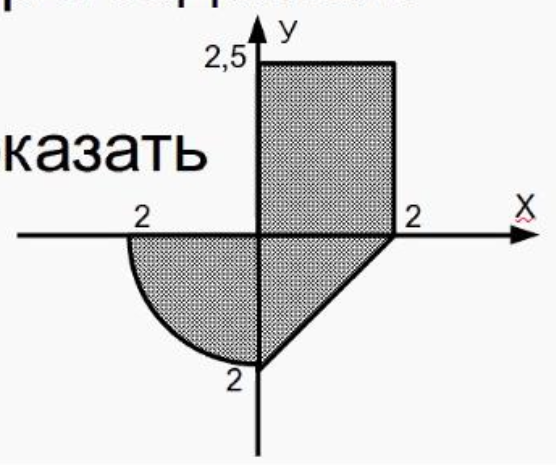
\includegraphics[width=.3\textwidth]{fig.png}\\
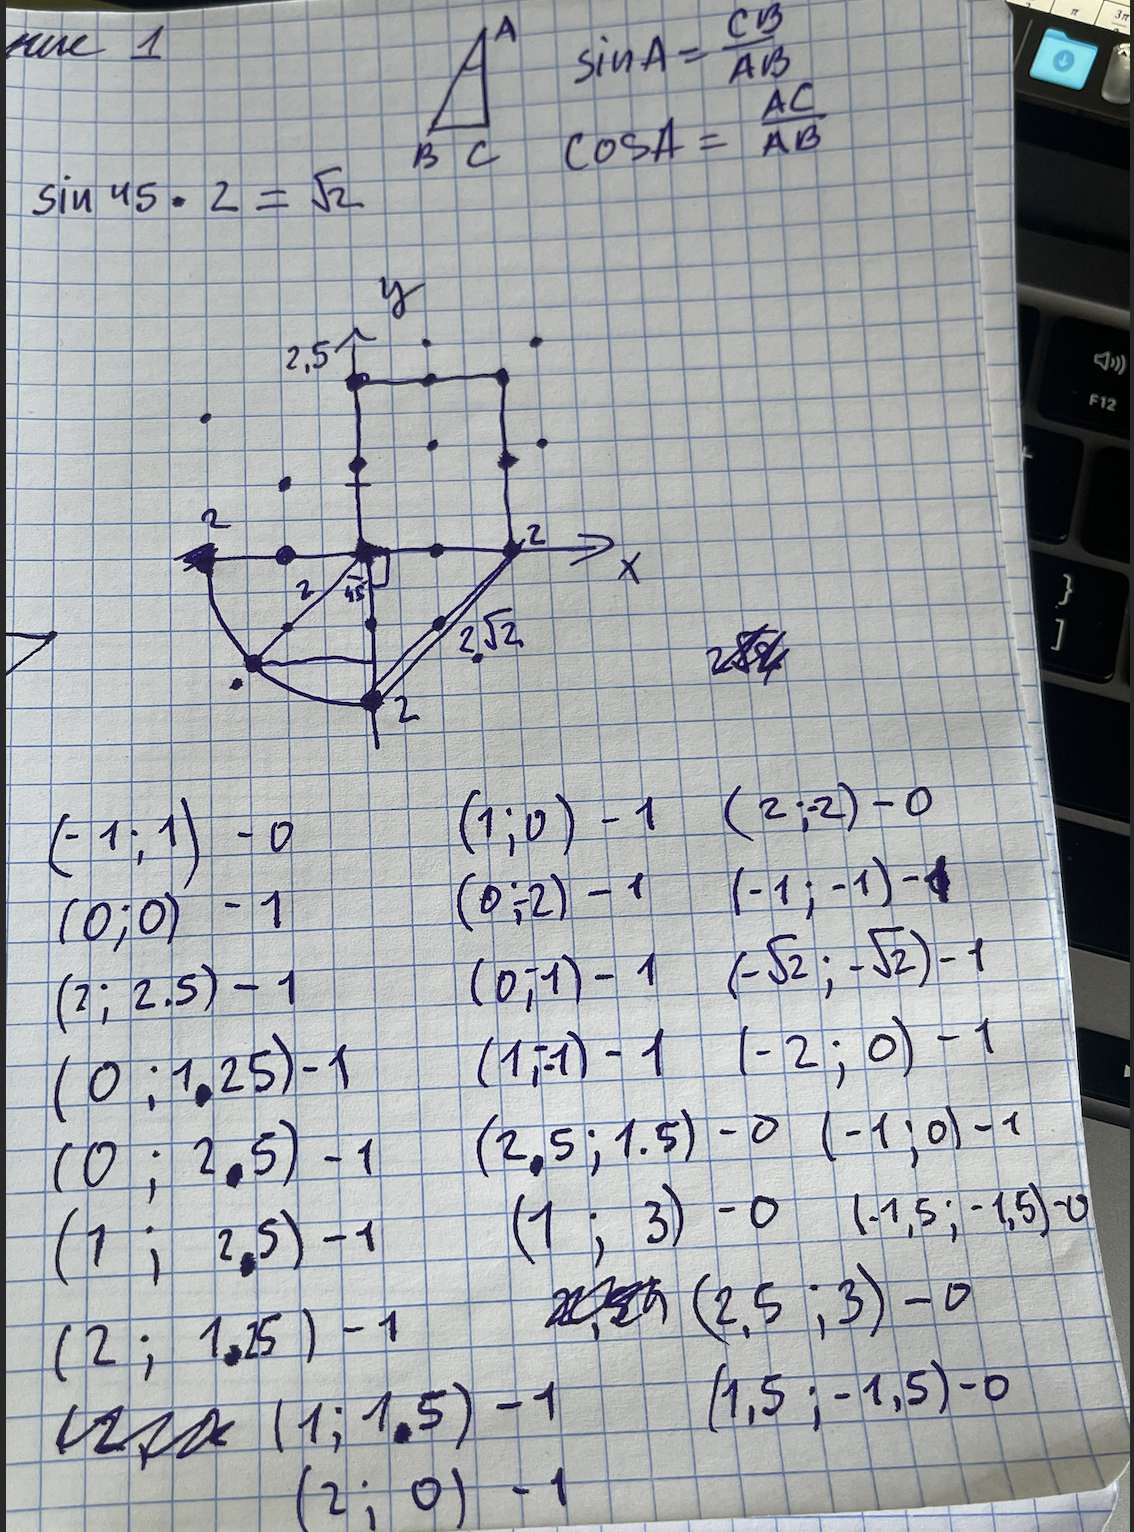
\includegraphics[width=.4\textwidth]{ris}

\subsection{Ресурсные риски}
Какие из перечисленных ниже рисков являются примерами ресурсных рисков? (перечислить номера вариантов ответа)

1. Риск поломки оборудования разработчкиов.

2. Риск возникновения конфликта между менеджером исполнителя и заказчиком.

3. Риск отсутствия необходимых кадров при переносе производства в другой город.

4. Риск отсутствия спроса на произведенную продукцию.

5. Риск запрета продажи автомобилей с ДВС для снижения негативного экологического воздействия на планету
\\
Ответ: 

1. Риск поломки оборудования разработчкиов.

3. Риск отсутствия необходимых кадров при переносе производства в другой город.

\subsection{Топ - 3 рисков по экспозиции}
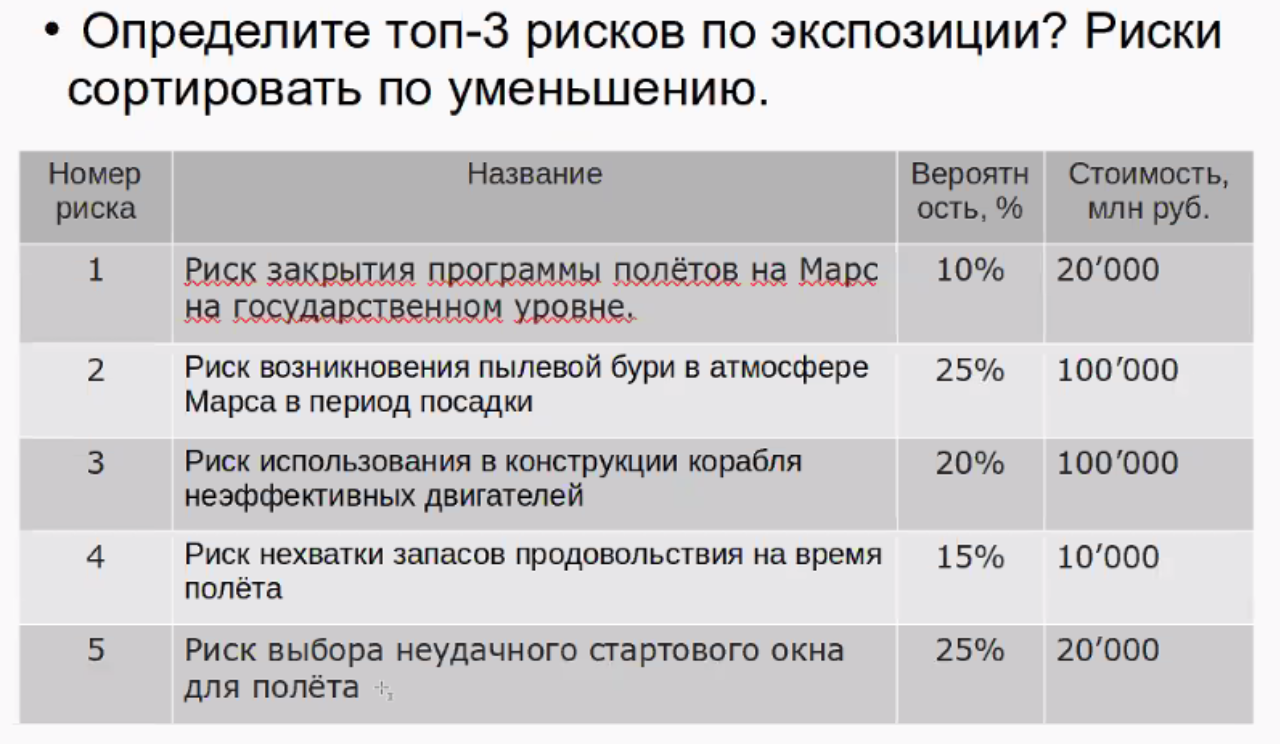
\includegraphics[width=.4\textwidth]{risk.png}
\\
Вероятность натсупления * потери = экспозиция
\begin{itemize}
    \item 0.1 * 20000 = 2000
    \item 0.25 * 100000 = 25000
    \item 0.2 * 100000 = 20000
    \item 0.15 * 10000 =1500
    \item 0.25 * 20000 = 5000
\end{itemize}
Ответ: 235

\subsection{Git pull}

Какие действия выполняет команда git pull

Ответ: скачать и применить к своему локальному репозиторию последнюю версию удаленного репозитория

\subsection{Git сommit}

Приведите команды, которые приведут к записи в репозиторий проекта нового коммита, содержащего файлы А,С,Е
\\ \\
git reset HEAD D

или git restore --staged D

git add C

git commit -m “commit0”
\\ \\
\\ \\
svn revert D

svn add C

svn commit -m ""
\subsection{Классификация проблемных ситуаций}
К какой категории классификации проблемных ситуаций жизненного цикла ПО с точки зрения тестирования относится приведённый ниже пример?

"Программист 3 категории Харитонов Фотий Аркадьевич, придя утром на работу в плохом настроении, заявил своим коллегам, что он их всех ненавидит, и случайно добавил в свою программу некорректно работающий код".

\begin{itemize}
    \item Mistake (Error) — ошибка, просчёт (человека).
    \item Fault — дефект, изъян (ПО в результате ошибки). Неверный шаг в алгоритме. Следствие ошибки.
    \item Failure — неисправность, отказ, сбой (внешнее проявление дефекта). Крах, падение программы.
    \item Error — невозможность выполнить задачу с использованием программы.
    \item BUG — используется неформально (они не подходят друг к другу). Может обозначать: дефект, отказ, невозможность выполнить задачу.
\end{itemize}
Ответ: mistake

\subsection{Скрипт сборки Gradle}

Приведите скрип сборки для Gradle, который устанавливает следующую последовательность целей сборки COMP, RESOURSE,
LIB, BUILD, DEPLOY. Цели печатают на констоли только свое имя.

Gradle:
\begin{verbatim}
    task COMP { doLast { println("COMP") } }
    task RESOURCE { doLast { println("RESOURCE") } }
    task LIB { doLast { println("LIB") } }
    task BUILD { doLast { println("BUILD") } }
    task DEPLOY { doLast { println("DEPLOY") } }
    build.dependsOn COMP, RESOURCE, LIB, BUILD, DEPLOY
\end{verbatim}

Make:
\begin{verbatim}
    .PHONY: all COMP RESOURCE LIB BUILD DEPLOY
    all: COMP RESOURCE LIB BUILD DEPLOY
    COMP: @echo "COMP"
    RESOURCE: @echo "RESOURCE"
    LIB: @echo "LIB"
    BUILD: @echo "BUILD"
    DEPLOY: @echo "DEPLOY"
\end{verbatim}

Ant:
\begin{verbatim}
    <project name="example build script">
    <target name="COMP">
    <echo message="COMP"/>
    </target>
    <target name="RESOURCE">
    <echo message="RESOURCE"/>
    </target>
    <target name="LIB">
    <echo message="LIB"/>
    </target>
    <target name="BUILD">
    <echo message="BUILD"/>
    </target>
    <target name="DEPLOY">
    <echo message="DEPLOY"/>
    </target>
    </project>
\end{verbatim}

\subsection{Тестовое покрытие}

Программисты Банка "Ваше Богатство" определяет тестовое покрытие для функции вычисления размера процентов на остаток по счету клиента. 
При наличии на счете от 50 000 до 100 000 руб. ежемесячно начисляется сумма эквивалентная 5.5\% годовых; 
если на счете от 100 001 до 500 000 то 4\%;
если больше 500000 то 0.01\%. 
При наличии на счете меньше 50 000 руб., проценты не начисляются. 
Сколько эквивалентных участков должно содержать тестовое покрытие, если в функцию могут поступать только корректные числовые данные?
\\ \\
Ответ: 4

\subsection{Простой системы}

Разработчик информационной системы заявил, что готовность его системы составляет 99.92\%. 
Какое максимальное целое количество минут в невисокосный год данная система может простаивать?

$365 \cdot 24 \cdot 60 \cdot (1-99.92)/100 = 420.48 = 420$

\subsection{Скорость работы системы}

Программа вычисляет значение по алгоритму, 
обрабатывая данные на уровне процессора (1 команда = 1 нс), уровне кэш-памяти второго уровня (20 нс), оперативной памяти (100 нс), ssd (50мкс). 
Для вычисления значения алгоритма используются 1000 команд на уровне процессора, 100 обращений к памяти, из которых 90\% кешируются в кэш-памяти второго уровня, а также 4 обращения к диску. 
На сколько процентов увеличится скорость работы алгоритма, если программист смог уменьшить количество обращений к SSD до одного раза? Ответ выразить в процентах.
\\
Ранее: $1000 \cdot 1 + (100/100 \cdot (100-90)) \cdot 100 + (100/100 \cdot 90)\cdot 20 + 4\cdot 50\cdot 10^3 = 203800 нс$
\\
Будет: $1000 \cdot 1 + (100/100 \cdot (100-90)) \cdot 100 + (100/100 \cdot 90)\cdot 20 + 1\cdot 50\cdot 10^3 = 53800 нс$
\\
\[\frac{203800-53800}{203800} \cdot 100 = 73\%\]

\[\frac{53800}{203800} \cdot 100 = 378\%\]
\section[Рубеж]{Вариант - 2}
\subsection{Доменная модель}
\subsection{Чему уделялось внимание в спиральной модели}

Применялась для разработки больших программных продуктов. После постановки целей и выявления альтернативных решений, производился анализ рисков для минимизации числа дествий для разработки ПО. На каждой итерации модели перед созданием прототипа происходит сверка с картой рисков. (При этом анализировались не только технические риски, но и политические и тд)
Так же в данной модели все изменения, которые вносятся в проект, являются неотъемлемой частью разработки. Любые действия с ними зависят от тех рисков, которые они несут для процесса разработки.




\section[Термины]{Термины}
\subsection[Модель требований FURPS+]{Модель требований FURPS+}
Подробное описание того что должно быть реализовано системой, но при этом не должно описывать, как его нужно реализовать.
Включает в себя функциональные требования, нефункциональные. 

Функциональные определяют, что система должна делать: наборы функциональных требований (FR + номер), возможности ПО (СAP + номер), требования к безопасности (SEC + номер).
Наборы - набор свойств продукты необходимый для выполнения конкретной деятельности (сис должна обеспечивать ввод, модификацию и удаление данных о клиенте).
Требования к безопасности - метод аунтификаци, список ролей, шифрование, хранение данных в защищённых источниках (сис должна обеспечивать двухфакторную аутентификацию пользователей с помощью имени пользователя и пароля и подтверждения с помощью СМС.)

Нефункциональные: 

Usaility - учёт особенностей пользователя (быстрота ответа в интервале), эстетические требавания (цвет, расстояния между элементами), согласованность пользовательсткого интерфейса, согласованность пользовательского интерфейса, требования к справочной подсистеме, требования к пользовательской документации, требования к учебным материалам.

Reliability - частота и обработка заказов, способность системы восстанавливать продуктивное функционирование, предсказуемость поведения, точность, среднее время между отказами. Требования к надёжности, которые предназначены для способности ПО безотказно функционировать. 
В требованиях обычно указывается допустимое число отказов и сбоев за определённый промежуток времени. Способность системы восстанавливать продуктивное функционирование в течение заданного времени.
Требованием является accuracy - точность, например, проведения вычислений. Коэффициент готовности системы — отношение времени исправной работы к сумме времён исправной работы и вынужденных простоев объекта, взятых за один и тот же календарный срок.

Performance - скорость решения задач, эффективность, готовность системы к решению задач, пропускная способность, время отклика, время восстановления, использование системных ресурсов.
Требованием является скорость решения вычислительных задач. Также скорость важна в длительных инженерных расчетах, когда необходимо выполнить, например, моделирование за разумное для человека время.
Требования к эффективности фиксируют процент времени, которое тратится на выполнение полезных задач, по отношению к времени на выполнение общесистемных.
Требованием к производительности является готовность (availability) быстро начать выполнение задачи.
Какой объём данных или запросов система может обработать за единицу времени.
Для большой реактивности придется пожертвовать пропускной способностью.

Supportability - способность системы к расширению и масштабированию и выполнению большего объема обработки данных. Адаптируемость под конкретные задачи, поддерживаемость.
Требования к совместимости позволяют использовать различные операционные системы, версии продуктов, браузеров и пр. совместно с разработанным ПО. Отдельно выделяются системные требования и минимальные требования к установке системы, например, объём
ОЗУ, количество и частота процессоров и пр.

\subsection[Доменная модель]{Доменная модель}
Доменная модель — это концептуальная модель предметной области, которая отображает ключевые сущности, их атрибуты и взаимосвязи между ними, а также основные правила бизнес-логики. Эта модель помогает разработчикам и всем участникам проекта лучше понять структуру и функционирование системы, на которой они работают.
Основной сущностью является класс, он включает только атрибуты без типов данных и без методов. Первая часть содержит имя класса, вторая содержит атрибуты.
\\ Типы отношений:

Ассоциация - это основные отношения между двумя сущностями. Эти сущности могут существовать независимо друг от друга. Мы рисуем его как простую сплошную линию.
Первая сущность имеет ссылку на другую, а другая - на первую. Мы можем изменить это поведение, добавив простую стрелку, определяющую направление отношений. Только экземпляр, из которого стрелки хранят ссылку на другую сущность в этих случаях.
\\
\begin{center}
    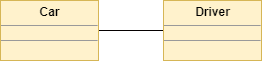
\includegraphics[width=.2\textwidth]{assoch.png}  
\end{center}

Агрегация - связь между классом и его частями. Бриллиант рисуется в классе, представляющем целое (например, раздел article - статья).
\begin{center}
    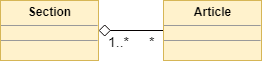
\includegraphics[width=.2\textwidth]{agreg.png}  
\end{center}

Композиция - тоже агрегирование, но часть не имеет смысла без главной сущности, при удалении сущности, удаляется и его часть
\begin{center}
    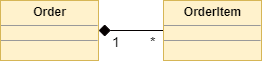
\includegraphics[width=.2\textwidth]{sostav.png}  
\end{center}

Обобщение - наследование. Одна сущность наследует свойства и поведение от другой сущности.
\begin{center}
    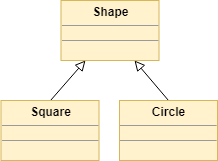
\includegraphics[width=.2\textwidth]{extends.png}  
\end{center}

Пример:
\begin{center}
    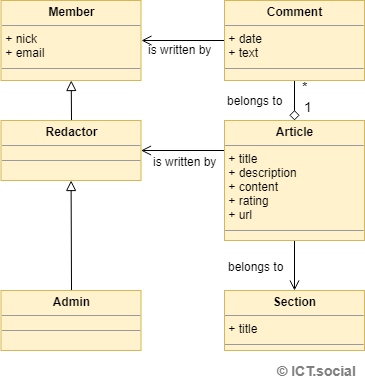
\includegraphics[width=.4\textwidth]{domenex.png}  
\end{center}

\subsection{Риски}

\begin{itemize}
    \item Прямые и непрямые - можем контролировать или управлять или нет. Прямыми рисками можно в явном виде управлять: воздействовать на них, уменьшать их вероятность, реагировать на них. Непрямые риски возникают по внешним причинам и не поддаются управлению, можно только принять на себя их последствия. Отсюда существуют различные методы работы с прямыми и непрямыми рисками.
    \item Ресурсные - организационные, финансовые, люди, время. связаны с недостатком у компании времени, людеи, денег, оборудования. Ути риски имеют отношение к особенностям и специфике конкретной организации, разрабатывающей проект. Данные риски являются управляемыми, так как возможно изменение выделяемых ресурсов.
    \item Бизнес-риски - конкуренция, подрядчики, убыточность решения. появляются из-за взаимодействия с другими организациями и рынком в целом. Они определены конкуренцией, взаимодействием с подрядчиками или потенциальной убыточностью решения, т.е. отсутствием в дальнейшем прибыли от реализации и внедрения ПО. Управление бизнес-рисками сложно поддается управлению со стороны разработчиков.
    \item Техничекие риски - границ проекта, технологические, внешние зависимости. находятся в пределах компетенции разработчиков и поэтому являются ими управляемыми. Примеры технических рисков - отсутствие у разработчиков компетенции в применяемых технологиях.
    \item Форс-мажор. В отличие от политических рисков, повлиять на форс-мажор нельзя, и предугадать его тоже. К таким рискам относятся стихийные бедствия, изменение законодательства и т.п.
    \item Политические риски - связаны с изменением сфер влияния внутри компании-заказчика.
    Например, с появлением нового менеджера могут измениться условия сделки. Это возможно предвидеть, но не всегда. Противодействием может быть упреждающая реакция на возможные изменения в компании (например, установление контактов с вероятным новым менеджером).
\end{itemize}

\subsection{Git rules}

\subsubsection{Определение}
Git - децентрализованная система. У каждого разработчика есть локальная копия репозитория, в котором хранится всё о проекте целиком и доступна вся история изменений, как от самого разработчика, так и история изменений других разработчиков.
Каждый локальный репозиторий имеет свой URL, по которому он доступен, а другие разработчики погут обращаться к нему при помощи алиасов. 
Благодаря такому подходу можно гибко подбирать вариант работы: 

централизованный рабочий процесс (главная репа и с ней синхронизируются все разработчики); 

рабочий процесс с менеджером по интеграции (каждый разраб меняет свой канонический репозиторий, открытый только для чтения, в локальной копии и потом запрашивает менеджера загрузить его в канонический реп);

рабочий процесс с диктатором и лейтенантами (лейтенанты - интеграционные менеджеры, которые отвечают за отдельный части репозитория. У всех лейтенантов есть ещё один интеграционный менеджер - доброжелательный диктатор, репозиторий которого выступает как эталонный, откуда все участники проекта получают изменения)

\subsubsection{Commands}
\begin{itemize}
    \item git pull - скачать и применить к своему локальному репозиторию последнюю версию удаленного репозитория
    \item git clone - клонировать удаленный репозиторий в новую директорию на локальной машине
    \item git init - создать новый пустой репозиторий Git или реинициализировать существующий
    \item git add - добавляет изменённые файлы к последующему коммиту, помещая их в Stage Area.
    \item git commit - фиксирует изменения в текущей ветке. Опция -т задает сообщение коммита, которое будет показываться пользователю
    \item git push - отправить коммиты из локального репозитория в удаленный репозиторий
    \item git status - показывает статус текущих состояний файлов в файловой системе и информацию о ветви, в которой производится редактирование.
    \item git log - показывает журнал коммитов, а опция -grah выводит в графическом виде ветви, в которых производились данные изменение.
    \item git branch — показывает ветви.
    \item git checkout — переключает разработчика между ветвями.
    \item git merge — объединяет несколько ветвей в текущую ветвь.
    \item git diff - покажет все изменения, которые были сделаны относительно последних зафиксированных изменений.
    \item git reset - отменить изменения, вернув файлы в рабочем каталоге к состоянию последнего коммита
    \item git fetch - скачать изменения из удаленного репозитория, но не применять их к локальному репозиторию
    \item git rebase - перенести или перепроиграть коммиты на другую базовую точку
    \item git cherry-pick - применить изменения из указанного коммита в текущую ветку
    \item git reset --hard HEAD сбросит все изменения, которые были сделаны в текущем локальном репозитории.
\end{itemize}


\subsection{SVN rules}

\subsubsection{Определение}
SVN - централизованная система контроля версий. Каждая фиксация изменений - ревизия. 
Организация файлов: есть каталоги проектов, внутри которых размещены директории, предназначенные для организации работы с разными версиями проекта. В каталоге trunk происходит основной процесс разработки. Для хранения истории релизов можно копировать содержимое trunk в доп каталоги trunk и tags.  
\begin{itemize}
    \item trunk - основная ветвь разработки
    \item branches - хранение модификаций продукта (Releases - значимые версии продукта, features - выполнение работ над версиями проекта без влияния на trunk, vendor - версии с модификациями сторонних библиотек)
    \item tag - функционально целостные изменения.
\end{itemize}


\subsubsection{Основной цикл разработчика}
\begin{itemize}
    \item svn checkout - первоначальное создание рабочей копии
    \item svn update - обновить рабочую копию
    \item svn (add, delete, copy, move, mkdir) - изменения в проекте 
    \item svn diff, svn status - просмотр изменений
    \item svn revert - откат изменений
    \item svn update - для загрузки изменений 
    \item svn commit - фиксация изменений
    \item svn merge - подгружает изменения из веток в рабочую копию, учитывая изменение структуры.
\end{itemize}

\subsection{Классификация проблемных ситуаций}

\begin{itemize}
    \item Mistake (Error) — ошибка, просчёт (человека).
    \item Fault — дефект, изъян (ПО в результате ошибки). Неверный шаг в алгоритме. Следствие ошибки.
    \item Failure — неисправность, отказ, сбой (внешнее проявление дефекта). Крах, падение программы.
    \item Error — невозможность выполнить задачу с использованием программы.
    \item BUG — используется неформально (они не подходят друг к другу). Может обозначать: дефект, отказ, невозможность выполнить задачу.
\end{itemize}

\subsection{Use-Case}
РАМКА БЕЗ АКТОРОВ!\\
Включение (Include) — обязательная, неотъемлемая связь между use-кейсами.\\
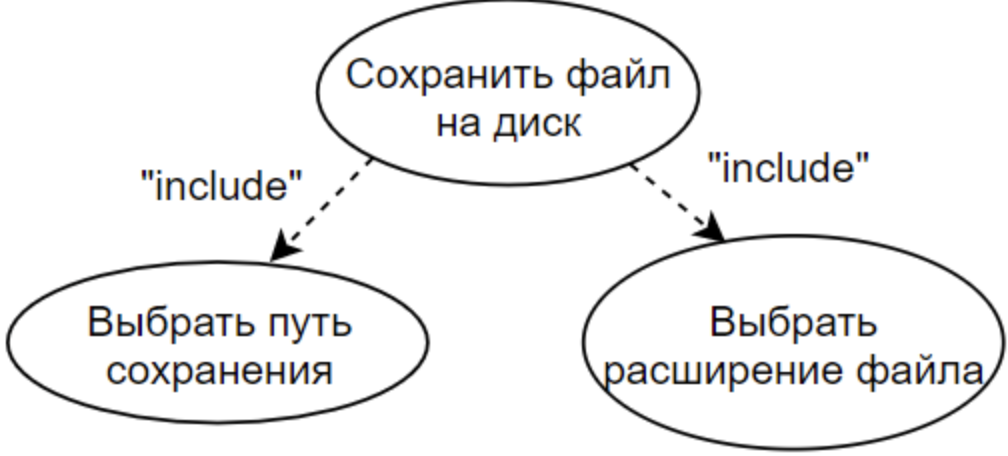
\includegraphics[width=.3\textwidth]{include.png}\\
Расширение (Extend) — необязательное отношение. Если use-кейс не является обязательным, то актор может выбирать.
\\ 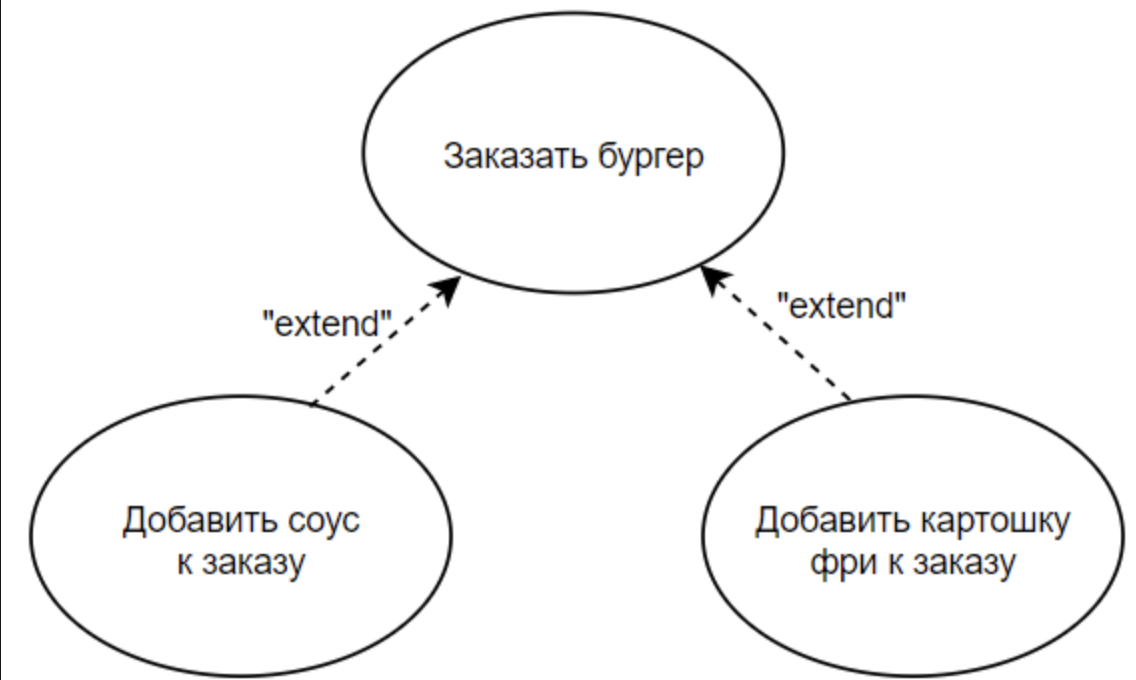
\includegraphics[width=.3\textwidth]{extend.png}\\
Отношение обобщения\\
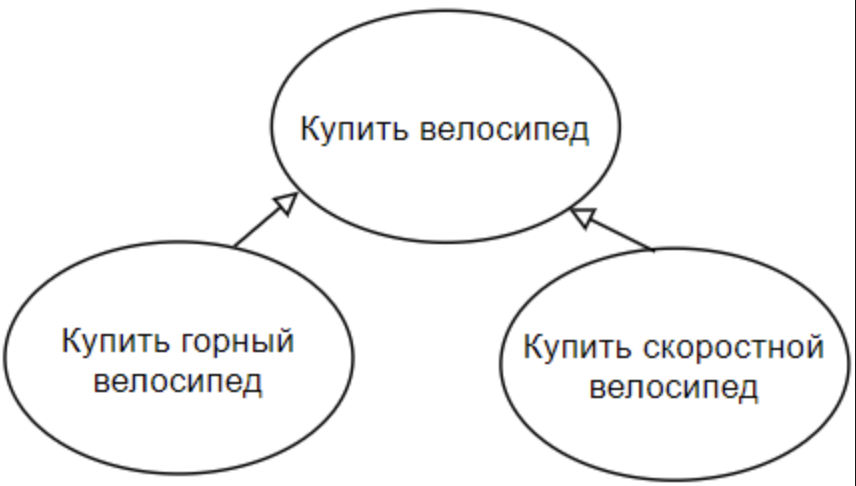
\includegraphics[width=.3\textwidth]{obob.png}\\
Отношение ассоциации\\

\includegraphics[width=.3\textwidth]{assos.png}

\subsection{Методологии разработки}

\subsubsection{Водопадная (Каскадная)}
Стандартные шаги разработки

\begin{itemize}
    \item Определение системных требований
    \item Определение требований в ПО
    \item Анализ требований
    \item Проектирование программы
    \item Разработка кода
    \item Тестирование
    \item Введение ПО в эксплуатацию
\end{itemize}

Есть понятие итерации между фазами разработки, есть возможность отката к предыдущей фазе. 
На фазе тестирования можно обнаружить, что итоговые характеристики отличаются от заданных изначально, поэтому нужно менять либо требования, либо дизайн системы. 
Возможно неверно определены требования, поэтому есть откат с фазы проектирования программы к определению требований в ПО.
\subsubsection{Методология Ройса}
Ройса предложил разбиение на следующие шаги:
\begin{itemize}
    \item Предварительный дизайн - занимаются только дизайнеры, цель: спроектировать, определить и создать модели обработки данных, даже если они будут требовать переделок. Разработать док - обзор будущей системы
    \item Документирование дизайна, которое включает: требования к системе, спецификация предварительного
    дизайна, спецификация дизайна интерфейсов, финальные спецификации дизайна системы, план
    тестирования, инструкция по использованию.
    \item Just do it nike tw - Предлагается запустить тестовую разработку параллельно основному процессу и взять это за каскадёра с сокращённым временем разработки, который позволит подтвердить основные хар-ки ПО или найти ошибки. 
    \item Тестирование - наиболее рискованная и дорогостоящая фаза, а также последний шанс для выбора альтернатив. Также при планировании тестирования исключается дизайнер и осмотр всех логических путей проводит другое лицо для инспекции кода. После исправления ошибок нужно провести checkout (тестирование)
    \item Подключение пользователя - это должно произойти на ранних этапах перед финальной поставкой продукта. Необходимо 3 точки: опыт, оценка и подтверждение пользователем - предварительный, критический и финальный просмотр.
\end{itemize}

\subsubsection{Традиционная V-chart model 1977}
Так как в то время уделялось внимание качеству ПО, то Ройсом была предложена идея. В основе V-chart model лежит такая же последовательность шагов как и в водопадной модели, но каждому уровню разработки положен свой уровень тестирования. Модульное, интеграционное и системное тестирование проводятся последовательно на основе критериев, которые заданы соответствующими уровнями разработки. Последний этап - приёмочное тестирование (проверка продукта на соответсвие функциональным требованиям).
Для тестирования нужно эталонное поведение, которое должно быть задано вне кода данной системы.
Есть разделение на статическое и динамическое тестирование. Динамическое - компьютерное исполнение тестов, а статическое (может проверяться на ранней стадии проекта, что позволяет выявлять грубые ошибки в проекте на начальной стадии) проверяет артефакты без компьютерного исполнения. 

\subsubsection{Многопроходная модель}

Учитывая сложность разработки проекта в один проход, было предложено разбить продукт по разным техническим и функциональным требованиям, а в последствии разрабатывать, реализовывать и интегрировать воедино в несколько проходов ввиде отдельных сборок. (инкременты)
Такой подход снижает стоимость изменений требований заказчика. Разработка - более управляема. 
Можно использовать уже частично разработанную систему. Современные Agile опираются на итеративный подход. Прогресс виднее заказчику.
Минусы: т.к. система может устаревать, то нужно обновлять её, но для инкрементной модели нужна неизменяемая архитектура и API (так как тут разработка ведётся параллельно несколькими командами), которые определяются в самом начале построения проекта (поэтому всё тяжело и дорого).
Документы по сборкам сложно поддерживать из-за быстрой скорости изменений.
Ещё сложно заключать контракты на разработку, так как там нужно фиксировать часы и суммы на разработку этапов.

\subsubsection{Модель прототипирования}

В данной модели лежит идея разделения процесса разработки проекта на прототипы, каждый из которых уточняет архитектуру, опираясь на функциональные требования. В начале система похожа на каркас, куда будет наращиваться проект. Относится к эволюцонному построению ПО.
Сначала планируется вся итерация, где проводится анализ текущих требований и подходов их реализации. Создаётся бд и интерфейс для пользователя, разрабатывается функционал и проверяется вместе с пользователем системы. Проводятся тесты. Если пользователю всё нравится, то происходит переход к конечной версии разработки ПО. 
Если пользователь не доволен, то разрабатывается ещё один прототип с новым интерфейсом и с бд. Прототипы создаются пока пользователь не протестирует все характеристики. 
В современных методах разработки променяются мокапы для создания простеньких визуальных моделей. Или применяют UX - модели, которые более сложные, но могут дать понять пользователю удобство пользования. 

\subsubsection{Spiral model}

Применялась для разработки больших программных продуктов.
Каждый виток спирали представляет собой одну фазу разработки очередной версии ПО. Сначала производится постановка целей, ограничений для каждой итерации. 
После постановки целей и выявления альтернативных решений, производился анализ рисков для минимизации числа дествий для разработки ПО. На каждой итерации модели перед созданием прототипа происходит сверка с картой рисков.
(При этом анализировались не только технические риски, но и политические и тд). После анализа рисков происходит разработка и валидация ПО. В конце последней итерации повторяется часть V-образной модели, где происходит тестирование разработанного ПО.
НА последней части каждого витка происходит планирование следующей итерации. 
В зависимости от фазы планированию подлежат действия по разработке требований и жизненного цикла разработки, собственно сама разработка, а также действия по интеграции
разработанных частей в единое целое и проведение тестирования.
Так же в данной модели все изменения, которые вносятся в проект, являются неотъемлемой частью разработки. Любые действия с ними зависят от тех рисков, которые они несут для процесса разработки.

\subsubsection{RAD методология}

Методология базируется на идеи увеличения участия пользователя в процессе разработки, а также идеи об автоматизации процессов. Она состояла в том, что сначало производится проектирование, а затем при помощи средств автоматизации собирается ПО. ПРи этом пользователь принимает непосредтсвенное участие в процессе разработки при помощи средств автоматизации (например создавать простые функции и интерфейсы).
Минусы: разработка может усложняться за счёт автоматизации и внедрения пользователя, также некоторые интерфейсы могут быть не сильно продуманы. Плюсы: реализуется бизнес-функция "Нужно разработать уже вчера".

\subsubsection{*UP методологии}

Процесс представляет собой разработку ввиде инкрементно-эволюционного подхода. Процесс разработки разбит на фазы. Также присутствуют дисциплины - набор правил и указаний (необходимы для определённых задач, таких как тестирование или определение требований).
Все дисциплины сделаны для того чтобы организовать разработчиков, дать им подходы, чтобы каждая роль процесса разработки могла выполнять необходимые, требуемые от неё действия.
Всего фаз 4: Incection (начало), Elaboration (проектирование), Construction (создание продукта), Transition (внедрение на стороне заказчика)
В рамках итеративного подхода фазы могут делиться на итерации.
\end{document}
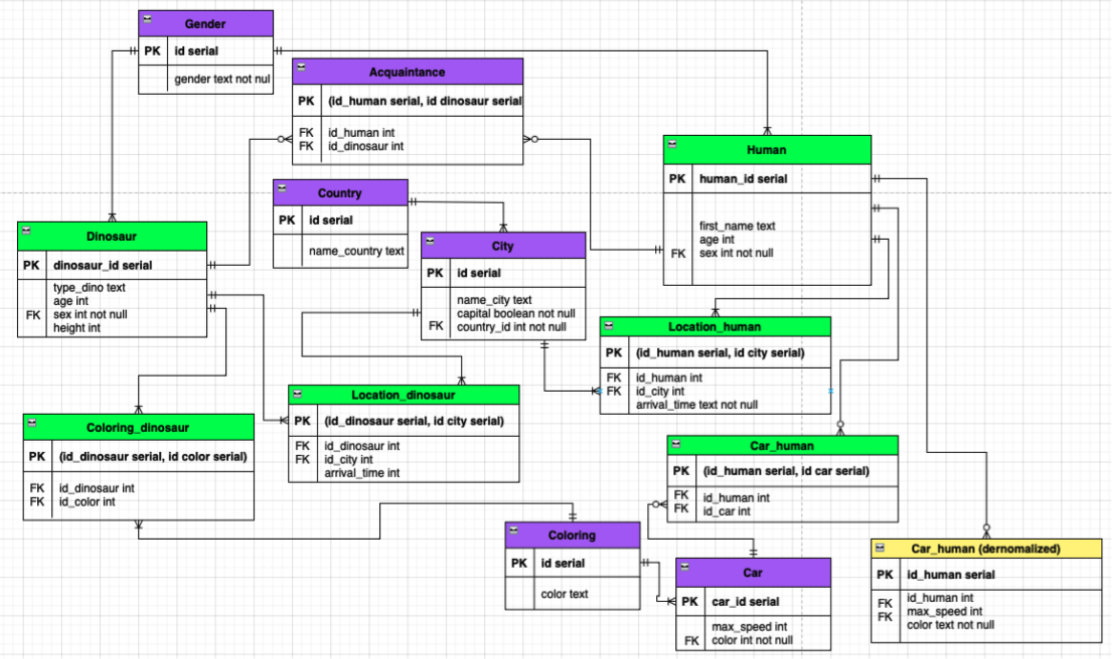
\includegraphics[width=.9\textwidth]{123}